%%
%% This is file `sample-sigconf.tex',
%% generated with the docstrip utility.
%%
%% The original source files were:
%%
%% samples.dtx  (with options: `sigconf')
%% 
%% IMPORTANT NOTICE:
%% 
%% For the copyright see the source file.
%% 
%% Any modified versions of this file must be renamed
%% with new filenames distinct from sample-sigconf.tex.
%% 
%% For distribution of the original source see the terms
%% for copying and modification in the file samples.dtx.
%% 
%% This generated file may be distributed as long as the
%% original source files, as listed above, are part of the
%% same distribution. (The sources need not necessarily be
%% in the same archive or directory.)
%%
%% The first command in your LaTeX source must be the \documentclass command.

\documentclass[sigconf,10pt]{acmart}

\acmConference{ISDS}{2020}{Garching bei Muenchen}
%%
%% \BibTeX command to typeset BibTeX logo in the docs
\AtBeginDocument{%
  \providecommand\BibTeX{{%
    \normalfont B\kern-0.5em{\scshape i\kern-0.25em b}\kern-0.8em\TeX}}}

%% Rights management information.  This information is sent to you
%% when you complete the rights form.  These commands have SAMPLE
%% values in them; it is your responsibility as an author to replace
%% the commands and values with those provided to you when you
%% complete the rights form.
\setcopyright{acmcopyright}
\copyrightyear{2020}
\acmYear{2020}
\acmDOI{isds}





%%
%% end of the preamble, start of the body of the document source.
\begin{document}

%%
%% The "title" command has an optional parameter,
%% allowing the author to define a "short title" to be used in page headers.
\title{YCSB vs BigBench}

%%
%% The "author" command and its associated commands are used to define
%% the authors and their affiliations.
%% Of note is the shared affiliation of the first two authors, and the
%% "authornote" and "authornotemark" commands
%% used to denote shared contribution to the research.
\author{Achraf Aroua}
\affiliation{%
  \institution{Technical University of Munich}
  \streetaddress{P.O. Box 1212}
  \city{}
  \state{}
  \postcode{}
}
\email{achraf.aroua@tum.de}


\author{Berkay Barlas}
\affiliation{%
  \institution{Technical University of Munich}
  \streetaddress{}
  \city{}
  \country{}}
\email{berkay.barlas@tum.de}




%%
%% By default, the full list of authors will be used in the page
%% headers. Often, this list is too long, and will overlap
%% other information printed in the page headers. This command allows
%% the author to define a more concise list
%% of authors' names for this purpose.

%%
%% The abstract is a short summary of the work to be presented in the
%% article.
\begin{abstract}
With the increase of data volume, velocity, and variety, we have seen the emergence of many systems that supports big data storage and data processing. Due to their different architectures, it has become necessary to evaluate and compare these systems. 
\newline
In this paper, we provide an overview of Yahoo! Cloud Serving Benchmark(YCSB) and BigBench, two big data systems benchmarks. We describe their design goals, workloads, and their architecture.
\end{abstract}


%%
%% Keywords. The author(s) should pick words that accurately describe
%% the work being presented. Separate the keywords with commas.
\keywords{Benchmark, YCSB, BigBench, Workloads, Design goals, Architecture}



%%
%% This command processes the author and affiliation and title
%% information and builds the first part of the formatted document.
\maketitle
\thispagestyle{fancy}
\section{Introduction}
The increasing data \emph{volume}, the requirement of quick data processing(\emph{velocity}), and the wide variety of data types(\emph{variety}) give various problems to traditional relational database management systems which are unable to solve. This led to the explosion of new systems with the goal of big data storing and processing. Despite their common goal, different decisions were made when implementing the systems to solve various problems faced in big data systems. For example, some systems are more optimized for writes while others have decided to optimize for reads.
The absence of a standard database benchmark caused database management systems developers to make performance claims based on self-defined and biased benchmarks. These specifically built benchmark tools are used to make misleading comparisons and claims. Therefore, benchmarks such as YCSB\cite{ycsb} and BigBench\cite{bigbench} emerged to tackle these issues and solve these problems by bringing standardized benchmark tools. 

The paper is organized as follows. Section 2 provides an overview of the design goals of YCSB and BigBench. Section 3 discusses the workloads of each benchmark in detail, while section 4 examines their architecture. Furthermore, section 5 gives a  comparison of the two benchmarks.Section 6 examines further work. Lastly, section 7 presents our conclusions.

\newline 

\section{Design Goals}
The Yahoo! cloud serving Benchmark was first presented in 2010 to evaluate and compare the performances of different cloud serving systems. These cloud systems are usually NoSQL systems that do not support ACID criteria.YCSB is used to evaluate the performance of cloud systems by examining their scalability and processing performance.
\newline
\newline
BigBench ,the first end-2-end benchmark tool for big data system , was first published in 2013. It is based on a fictional product retailer. BigBench focuses on parallel database management systems and map reduce engines.
Also, BigBench V2, an new  version of BigBench with improved workload queries and data generator, published in 2017.

\subsection{YCSB Tiers}
In this section, we will see the two different tiers of the YCSB benchmark that aims at  evaluating   the performance and the scalability of cloud serving systems 
\subsubsection{\textbf{Tier1:Performance:}} \hfill\\
Since cloud serving systems aim for supporting very high request rates, we try in this tier to see the latency of the system when it is under load. It is expected that the latency of the requests to increase when the number of throughput (the number of operations per second) increases. This can be mostly explained to the less space for disk, CPU, and so on. Thus, there is a trade-off between latency and throughput.


This performance tier helps in  examining  this trade-off for different database systems by measuring the latency as we increase the throughput until the system is saturated and throughput stops increasing 
\subsubsection{\textbf{Tier2:Scaling:}} \hfill\\ 

YCSB uses two metrics when evaluating the scaling aspect of different cloud serving systems:\newline
\textA-   \textbf{Scale-up}:
Here, we examine the change and the impact on performance when machines are added to the system. This can be easily checked when doing this following experiment: \newline
\emph{Part-1}
\begin{itemize}
\item {\verb|Step 1|}: Load data to a certain number of servers
\item {\verb|Step 2|}: Run the workload
\end{itemize}
 We try to save the results of this workload to use it later to compare it with the latter results.  \newline
  \emph{Part 2}
 \begin{itemize}
\item {\verb|Step 1|}: Delete data from servers
\item {\verb|Step 2|}: Add more servers
\item {\verb|Step 3|}: Load more large data
\item {\verb|Step 4|}: Run the workload
\end{itemize}
 In the end, we compare the results of this workload with the first one. If a system has good scaling properties, we will get constant performance. More importantly, to make this experiment fair, the number of server and amount of data should increase proportionally \newline
 \textA-  \textbf{Elastic speedup}:
 This metric is quite similar to the first scale-up metric. However, the key difference is to check the performance of databases when machines are added but while the system is running. This can also be checked with the following experiment :
 \begin{itemize}
\item {\verb|Step 1|}: Load data to a certain number of servers
\item {\verb|Step 2|}: Run the workload
\item {\verb|Step 3|}: Increase the number of servers
\end{itemize}
after we increased the number of servers, we can conclude if the system offers the elasticity properties. If there's a performance improvement in a short time, then this system is considered as elastic. Usually, Systems can not show this improvement instantly because it needs time to reconfigure itself due to the newly added servers.

\subsection{BigBench Design Goals}
As the number of big data applications increased different requirements arose which led to the development of different database management systems. Therefore, a standard comparison and benchmark system are required to evaluate different big data systems.  
\newline \newline
BigBench is designed as end to end benchmarking tool that covers all the events during the initialization and operation of big data system. 
\newline \newline
BigBench is created in cooperation with the University of Toronto, Oracle, Teradata, and Infosizing. It is adopted from another benchmarking tool TPC -DS which developed by Transaction Processing Performance Council (TPC)\cite{tpc}.
\newline \newline 
BigBench is based on a fictional product retailer system. Therefore, BigBench initializes and operates the database system as it is a product retailer  who sells products to customers via physical and online stores 

\section{Workloads}
\subsection{YCSB Workloads}
To conduct the tiers presented in the previous section, YCSB comes with several built-in workloads. A workload represents a particular mix of read/write operations, data sizes, request distributions, and so on. YCSB has a package called \textbf{Core Package} which is a collection of related workloads. Each of these workloads tries to examine and evaluate systems in a particular performance space. These workloads do not cover the entire performance space but the most relevant ones to a cloud serving system .Since cloud systems have some trade-offs like synchronous vs asynchronous reads, these workloads aim at evaluating them. However, the user can also define new workloads thanks to the extensibility of YCSB.  This process is defined in section 4. \newline
 
Despite their different properties, these workloads are just a variation of the same basic application. In this application, there is a table of records, each with F fields. Each record is identified just by a primary key like "user145143". The values of each field are random ASCII characters of length L. Then for each application, it exists L*F byte records at the total. 
 Against these data, each operation is randomly chosen to be one of: Insert, Update, Read, Scan.
Since YCSB deals only with cloud serving systems, the YCSB package contains different combinations of workloads that aims to model different cloud systems application. These workloads are shown below in \textbf{Table 1 }

\begin{table}[h!]
  \caption{Different workloads in  the \textbf{Core Package}}
  \label{tab:freq}
  \begin{tabular}{ccl}
    \toprule
    Workload & Operations & Record selection \\ \hline
    \midrule
       A- Update heavy & Read:50\%, Update:50\% & Zipfian \\ \hline
    B-Read heavy & Read:95\%, Update:5\% & Zipfian \\    \hline
    C-Read only & Read:100\% & Zipfian \\    \hline
    D-Read latest & Read: 95\%, Insert:5\% & Latest \\ \hline
    E-Short range & Scan:95\%, Insert:5\% & Zipfian/Uniform \\ \hline
  \bottomrule
\end{tabular}
\end{table}
\subsubsection{ \textbf{YCSB Distributions}} \hfill\\
\newline
Based on \textbf{Table 1}, the behavior of selecting a record is different from one workload to another. When running a workload, various random choices need to be done: which record to run, how many records to scan, which operation to perform, and many others. Thus, each of these workloads is associated with some random distribution. Fortunately, YCSB has several probability distributions :
\begin{itemize}
  \item \textbf{Uniform}: All random action have the same constant probability. An example would be when  choosing an operation, is that all operations have the same probability to be  performed
  \item \textbf{Zipfian}: In this distribution, some items will be extremely popular(the head of distribution) while others will be usually unpopular(the tail of the distribution)
  \item \textbf{Latest}: This distribution is a special case of the zipfian  where the most inserted items are the head of distribution
  \item \textbf{Multinomial}: Probabilities for each item are specified and assigned at the beginning. Thus each item has a constant specific probability to be chosen
\end{itemize}
Thanks to these different distributions, different applications behavior can now be mimicked by the workloads which can help us in benchmarking the systems.
\subsection{BigBench Workloads}
BigBench workload depends on 30 queries. And these 30 queries designed to cover business and technical functions. These workloads defines the queries that will be used to test data system.

\subsubsection{Business Dimension} \hfill\\
For business functions these workloads are designed cover the different categories of big data analytics proposed by McKinsey\cite{mckinsey}. BigBench covers 10 big data levers in 5 business category.
\begin{enumerate}
   \item Marketing
        \begin{itemize}
            \item Cross-selling
            \item Customer micro-segmentation
            \item Sentiment analysis
            \item Enhancing multi-channel consumer experience
        \end{itemize}
   \item Merchandising
        \begin{itemize}
            \item Assortment optimization
            \item Pricing optimization
        \end{itemize}
   \item Operations
           \begin{itemize}
            \item Performance transparency
            \item Return analysis
        \end{itemize}
   \item Supply chain
           \begin{itemize}
            \item Inventory management
        \end{itemize}
   \item New Business Models
           \begin{itemize}
            \item Price Comparison
        \end{itemize}
   \begin{itemize}
     \item The individual entries are indicated with a black dot, a so-called bullet.
     \item The text in the entries may be of any length.
   \end{itemize}
\end{enumerate}

\subsubsection{Technical Dimension} \hfill\\
For technical functions, these workloads are designed to span three different dimensions based on data sources, query processing types and analytic techniques.
\begin{enumerate}
    \item \textbf{Query Processing Type}
    \newline
    This technical function focuses on processing type of queries; declarative and procedural in addition to mixture of both. This means some queries are declarative can be used with SQL or procedural can be used with Map-Reduce while others are can be used with mix of both with a language like Pig Latin.
    
    \item \textbf{Data source dimension}
    \newline
    BigBench targets three different data types; structured, semi-structured and un-structured. Queries on web click events checks semi-structured and queries about product reviews check un-structured data. There are also some queries that works on multiple data types.
    
    \item \textbf{Analytic Techniques}
    \newline
    In this functionality BigBench workloads aims different business analytic methods. The three main areas used by defining queries are simple reporting, data mining and statistical analysis. 
\end{enumerate}

To summarize the workload queries in BigBench are defined according to business cases in a way that covers technical dimensions.  

\section{Architecture}
\subsection{ YCSB Client Architecture}
\begin{figure}[h!]
  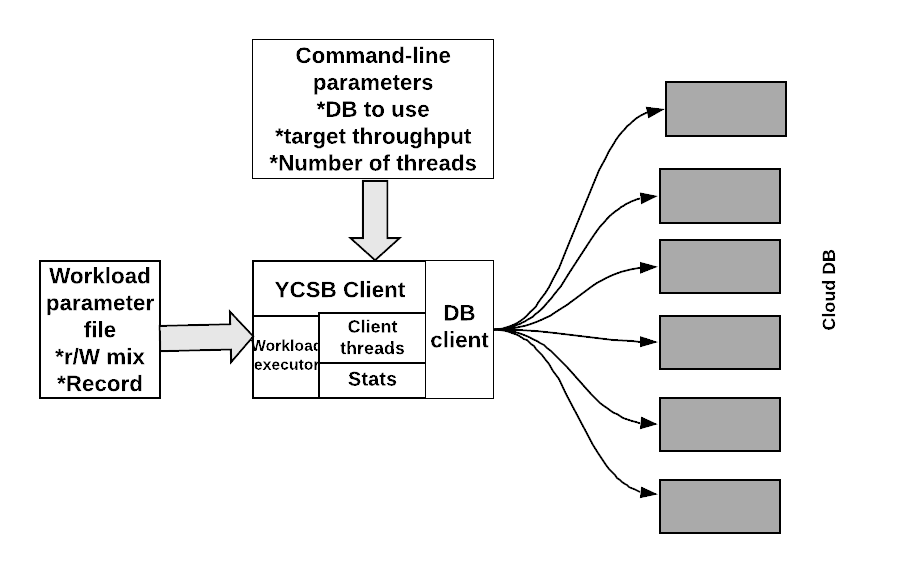
\includegraphics[width=\linewidth]{client.png}
  \caption{YCSB client Architecture}
  \label{fig:boat1}
\end{figure}
The YCSB client written in Java is a workload and data generator. It is responsible for generating data to be loaded to the database and the operations to be executed on them.
The client has different modules and its architecture can be seen in Figure 1.
The client has a command-line and a workload parameter file which are responsible for letting the user pass the parameters to the client. These parameters represents
\textbf{the workload } and \textbf{run-time properties} of the client. First, the workload properties are the read/write mix of the database, the distributions, and the number of records.  These properties can be shared among different experiments.
The run time properties are on the other hand are specific for a given experiment. This includes the database interface layer which is different for every system and the number of threads and so on.\newline
Furthermore, multiple threads are running inside the client. Each of these threads is responsible for executing a series of operations by making calls to the database interface layer. These calls can happen in two phases: First in \textbf{the load phase} when loading the data to the database and in \textbf{the transaction phase}  which corresponds to executing the workload. Moreover, these threads are also responsible for measuring the latency and the achieved throughput of the operations and report these results back to the statics module. Finally, the statics module aggregates the measurements and reports an average 95th and 99th\% latencies. The results are returned as either a histogram or a time series of reported latencies.
\subsection{YCSB Extensibilty}
Due to the various amount of different cloud serving systems, one of the key features of YCSB is that it is easily extensible. Therefore, developers can extend it to benchmark a cloud system different from the one originally supported by YCSB. As discussed in subsection 4.1 the database interface layer is responsible for translating requests from the client threads to the databases. Thus, you can extend the YCSB client  in order to benchmark new database systems   by writing a new class implementing the following methods:\textbf{read(), insert(), update(), delete(), scan()}.
These represent the \textbf{CRUD} methods which allow us to work with a new database system.
The user can also extend the client by defining new packages of new workloads in two ways. The most genuine way is to define a workload that uses \textbf{CoreWorkload} but with different parameters. By changing the parameters, the user can choose which operations to perform, which distribution to use and the number of records to include in the workload.
The second approach which is the harder way is to write a new Workload executor  Java class. With this approach, the user can perform complex operations and extend the workload to evaluate different points in the performance space. 

\subsection{BigBench’s Architecture}
BigBench data model d considers all important features of a big data system in terms of the three Vs, volume, variety, velocity described by Douglas Laney\cite{laney}: 
\newline \newline


\subsubsection{BigBench’s Data Model} \hfill\\
\newline
Bigbench is using an improved version TPC-DS data model. While the previous data model was only consisting of structured data, the new data model also includes a semi-structured data type for weblogs, and click stream events, and unstructured data type for product reviews. The improved data model is shown in Figure 2.
\newline 
Their design assumes
\begin{itemize}
\item The semi-structured data is in a key-value format which is similar to the log format of Apache’s web server.
\item The un-structured data used by product reviews doesn't require users.
\end{itemize}

\begin{figure}[h!]
  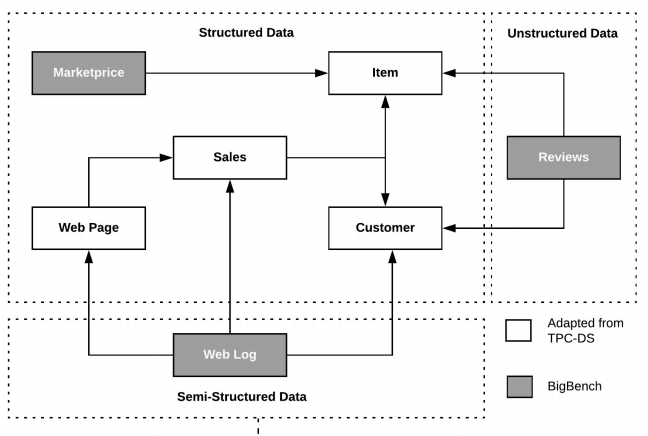
\includegraphics[width=\linewidth]{bb_datamodel.png}
  \caption{BigBench Data Model}
  \label{fig:boat1}
\end{figure}

\subsubsection{BigBench’s Data Generator} \hfill\\
\newline 
To test a big data system end-2-end, BigBench generates required data for benchmarking for 3 different data types. The data generator used in BigBench is an extended version of The Parallel Data Generation Framework (PDGF)\cite{pdgf}. PDGF is a parallel data generator tool implemented in Java and fully platform-independent for producing large amounts of data. Previously, it was only generating structured datatype, while, improved version supports semi-structured and un-structured data types.

\subsubsection{BigBench Review Generation} \hfill\\      

\begin{figure}[h!]
  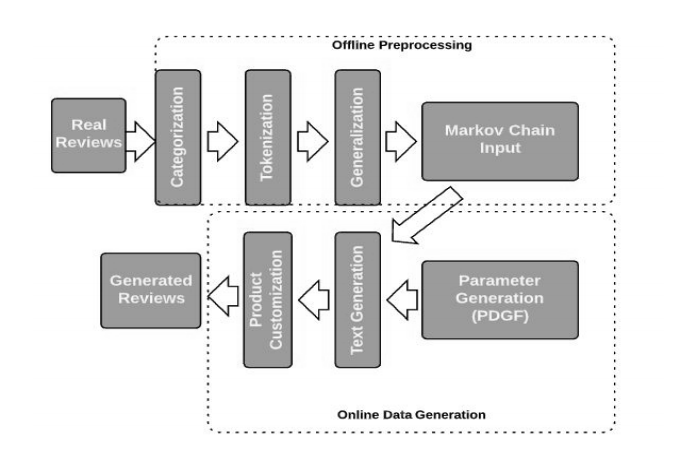
\includegraphics[width=\linewidth]{bb_reviewgen.png}
  \caption{BigBench Review Generation}
  \label{fig:boat1}
\end{figure}

Reviews are the unstructured type of data. To create a much more realistic data set they play a crucial role.
\newline
BigBench uses an algorithm called TextGen for review reproduction. The review generator developed for BigBench is another independent tool that can be modified using XML. It produces text reviews based on samples.
Their algorithm TextGen uses a Markov Chain method which creates a dictionary from the words in the given input. BigBench uses real product reviews from amazon.com for as initial sample data. Figure 3 shows the outline of the review production process.
\newline 
The review generation consists of two phases
\begin{enumerate}
   \item Reprocessing the data
   \item Online data generation
\end{enumerate}
The preprocessing part categorizes and prepares data to process with the Markov Chain algorithm. It creates a dictionary to be used in the review generation. The transition possibilities, Markov chains, of a word in the input reviews calculated. BigBench uses order-2 chains to generate product reviews.
\newline      
During the online data generation part, the generator uses products in the system to generate reviews according to produced parameters from PGDF.

\subsubsection{BigBench Metrics and Evaluation} \hfill\\
\newline 
BigBench doesn't have a final metrics design, on the other hand, it is suggested to use query execution times as a performance metric similar to TPC-DS. Instead of using specific queries using query processing type to categorize execution times will bring out the processing performance. \newline
BigBench is tool that focuses on database management systems and Map-Reduce engines, thus, any of these systems or combination of them should be able used in benchmark. Figure 4 shows an example architecture of DBMS system that BigBench can evaluate.

BigBench begins evaluation with creation of tables. It uses DSDGEN from TPC-DS to create structured data, and improved version of PDGF to create new parts in data model; web logs and products reviews. The generated data loads into tables with additional changes if required such as parsing web logs to create a schema. After loading the data, BigBench executes defined workload queries using an interface and execution times of each query are reported.  
\begin{figure}[h!]
  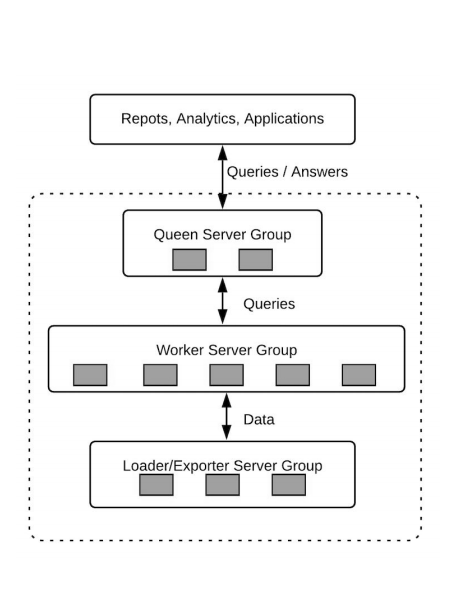
\includegraphics[width=\linewidth]{bb_evaulation.png}
  \caption{Example DMBS architecture for BigBench Evaluation}
  \label{fig:boat1}
\end{figure}

\section{Comparison}
YSCB and Bigbench are two benchmarking tools for big data systems. They are designed to create a standard comparison system.
\newline \hfill\\
Both of the benchmarking tools are open source and end-to-end benchmarks
\newline \hfill\\
However, YSCB and Bigbench have distinct features from each other which makes them useful for different situations. YCSB provides an apples to apples performance comparison of systems. It focuses on \emph{serving} systems that have different tradeoffs like read vs write performance. Therefore, YCSB tries to examine them directly with workloads that are mixes of OLTP(Online Transactional Processing) operations.
However, Bigbench is based on a fictional retailer. This means that it uses certain workload queries to evaluate data management systems which makes it a better solution for complex comparisons needed for particular applications. \newline

\section{Further work}
\subsection{YCSB++}
YCSB++ first presented in 2011, is a set of extension to YCSB framework. This benchmark is used to evaluate the advanced features of NoSQL systems like Bulk loading,fast ingest techniques and so on . These extensions are  \emph{multi tester coordination, eventual consistency  measurements, workloads multi phase workloads}  and they allow for more complex tests. One  important improvement would be parallel testing . In YCSB, at most one client can be run at once. However in YCSB++, we have a zookeper-based synchronisation for multiple client allowing the different tests to be coordinated

\subsection{BigBench V2}
BigBench V2 is published in 2017 as an improved version to solve drawbacks of BigBench. The data generator used in first version improved to produce structured, semi-structured and unstructured data types according to a scale factor in new version. The data model changed to simple star schema from previous complex schema to keep up with recent big data systems. 
In addition to these improvements, BigBench v2 assumes web logs are in key value format instead of converting them to structured type. 
\section{Conclusion}
In this paper, we explained the need for a tool that compares different cloud management systems and introduced two benchmarking tools for big data systems: YCSB and BigBench. After examining the metrics of each benchmark, this paper reviews their architecture and their workload generation technique. Additionally, by comparing the systems, we gave an overview of the two implemented improvements to the systems which are YCSB++ and BigBenchV2. 
\newline \newline
Over a decade YCSB became popular for benchmarking different cloud serving systems. Currently, YCSB is implemented and can be run with more than 18 different engines like \emph{Cassandra, HBase, MongoDB,} etc.\newline
\newline
BigBench also became one of the most known benchmarking tools due it's capabilities in realistic evaluation results. It's adopted as TPCx-BB by the Transaction Processing Performance Council.


\begin{thebibliography}{9}
\bibitem{bigbench}
A. Ghazal, T. Rabl, M. Hu, F. Raab, M. Poess, A. Crolotte, and H.-A. Jacobsen, 
\textit{BigBench: Towards An Industry Standard Benchmark for Big Data Analytics}.
in SIGMOD, 2013, pp. 1197–1208.

\bibitem{pdgf}
T. Rabl, M. Frank, H. M. Sergieh, and H. Kosch. 
\textit{A Data Generator for Cloud-Scale Benchmarking} In TPCTC, pages 41–56, 2010.

\bibitem{laney} 
D. Laney.
\textit{3D Data Management: Controlling Data Volume, Velocity and Variety.}.
Technical report, Meta Group, 2001.

\bibitem{mckinsey}
J. Manyika, M. Chui, B. Brown, J. Bughin, R. Dobbs, C. Roxburgh, and A. H. Byers. 
\textit{Big data: The Next Frontier for Innovation, Competition, and Productivity.} Technical report, McKinsey Global Institute, 2011.
\\\texttt{http://www.mckinsey.com/insights/mgi/research/
technology\_and\_innovation
/big\_data\_the\_next\_frontier\_for\_innovation/}

\bibitem{tpc}
TPC Benchmark DS
\bibitem{bigbench2}
Ghazal, Ahmad and Ivanov, Todor and Kostamaa, Pekka and Crolotte, Alain and Voong, Ryan and Al-Kateb, Mohammed and Ghazal, Waleed and Zicari, Roberto,
\textit{BigBench V2: The New and Improved BigBench}
10.1109/ICDE.2017.167, 2017, pp. 1225-1236.
\bibitem{ycsb} 
Benchmarking Cloud Serving Systems with YCSB
Yahoo! Research
Santa Clara, CA, USA
{cooperb,silberst,etam,ramakris,sears}@yahoo-inc.com
978-1-4503-0036-0/10/06
 \\\texttt{https://www2.cs.duke.edu/courses/fall13/compsci590.4//}

\bibitem{ycsbplus} 
YCSB++: Benchmarking and Performance Debugging Advanced Features in Scalable Table Stores. Swapnil Patil, Milo Polte, Kai Ren, Wittawat Tantisiriroj, Lin Xiao, Julio Lopez, Garth Gibson, Adam Fuchs, Billie Rinaldi. Proc. of the 2nd ACM Symposium on Cloud Computing (SOCC '11), October 27–28, 2011, Cascais, Portugal. Supersedes Carnegie Mellon University Parallel Data Laboratory Technical Report CMU-PDL-11-111, August 2011. \\\texttt{https://www.pdl.cmu.edu/ycsb++/}

\bibitem{benchmarking} 
Benchmarking Big Data Systems: A Review IEEE  TRANSACTIONS ON SERVICES COMPUTING, VOL. 11, NO. 3, MAY/JUNE 2018
University of Texas at Austin, Austin, TX 78712.
Digital Object Identifier no. 10.1109/TSC.2017.2730882
 \\\texttt{https://www.researchgate.net/publication/318664623}

\end{thebibliography}

































\end{document}
\endinput
%%
%% End of file `sample-sigconf.tex'.
